% Options for packages loaded elsewhere
% Options for packages loaded elsewhere
\PassOptionsToPackage{unicode}{hyperref}
\PassOptionsToPackage{hyphens}{url}
\PassOptionsToPackage{dvipsnames,svgnames,x11names}{xcolor}
% Code above from https://github.com/quarto-dev/quarto-cli/blob/main/src/resources/formats/pdf/pandoc/passoptions.latex
% Customization below
\PassOptionsToPackage{babel}{csquotes}
%
\documentclass[
  american,
  11pt,
]{stylisharticle}
\usepackage{xcolor}
\usepackage{amsmath,amssymb}
\setcounter{secnumdepth}{2}
\usepackage{iftex}
\ifPDFTeX
  \usepackage[T1]{fontenc}
  \usepackage[utf8]{inputenc}
  \usepackage{textcomp} % provide euro and other symbols
\else % if luatex or xetex
  \usepackage{unicode-math} % this also loads fontspec
  \defaultfontfeatures{Scale=MatchLowercase}
  \defaultfontfeatures[\rmfamily]{Ligatures=TeX,Scale=1}
\fi
\usepackage{lmodern}
\ifPDFTeX\else
  % xetex/luatex font selection
\fi
% Use upquote if available, for straight quotes in verbatim environments
\IfFileExists{upquote.sty}{\usepackage{upquote}}{}
\IfFileExists{microtype.sty}{% use microtype if available
  \usepackage[]{microtype}
  \UseMicrotypeSet[protrusion]{basicmath} % disable protrusion for tt fonts
}{}
\makeatletter
\@ifundefined{KOMAClassName}{% if non-KOMA class
  \IfFileExists{parskip.sty}{%
    \usepackage{parskip}
  }{% else
    \setlength{\parindent}{0pt}
    \setlength{\parskip}{6pt plus 2pt minus 1pt}}
}{% if KOMA class
  \KOMAoptions{parskip=half}}
\makeatother
% Make \paragraph and \subparagraph free-standing
\makeatletter
\ifx\paragraph\undefined\else
  \let\oldparagraph\paragraph
  \renewcommand{\paragraph}{
    \@ifstar
      \xxxParagraphStar
      \xxxParagraphNoStar
  }
  \newcommand{\xxxParagraphStar}[1]{\oldparagraph*{#1}\mbox{}}
  \newcommand{\xxxParagraphNoStar}[1]{\oldparagraph{#1}\mbox{}}
\fi
\ifx\subparagraph\undefined\else
  \let\oldsubparagraph\subparagraph
  \renewcommand{\subparagraph}{
    \@ifstar
      \xxxSubParagraphStar
      \xxxSubParagraphNoStar
  }
  \newcommand{\xxxSubParagraphStar}[1]{\oldsubparagraph*{#1}\mbox{}}
  \newcommand{\xxxSubParagraphNoStar}[1]{\oldsubparagraph{#1}\mbox{}}
\fi
\makeatother


\usepackage{longtable,booktabs,array}
\newcounter{none} % for unnumbered tables
\usepackage{calc} % for calculating minipage widths
% Correct order of tables after \paragraph or \subparagraph
\usepackage{etoolbox}
\makeatletter
\patchcmd\longtable{\par}{\if@noskipsec\mbox{}\fi\par}{}{}
\makeatother
% Allow footnotes in longtable head/foot
\IfFileExists{footnotehyper.sty}{\usepackage{footnotehyper}}{\usepackage{footnote}}
\makesavenoteenv{longtable}
\usepackage{graphicx}
\makeatletter
\newsavebox\pandoc@box
\newcommand*\pandocbounded[1]{% scales image to fit in text height/width
  \sbox\pandoc@box{#1}%
  \Gscale@div\@tempa{\textheight}{\dimexpr\ht\pandoc@box+\dp\pandoc@box\relax}%
  \Gscale@div\@tempb{\linewidth}{\wd\pandoc@box}%
  \ifdim\@tempb\p@<\@tempa\p@\let\@tempa\@tempb\fi% select the smaller of both
  \ifdim\@tempa\p@<\p@\scalebox{\@tempa}{\usebox\pandoc@box}%
  \else\usebox{\pandoc@box}%
  \fi%
}
% Set default figure placement to htbp
\def\fps@figure{htbp}
\makeatother


% definitions for citeproc citations
\NewDocumentCommand\citeproctext{}{}
\NewDocumentCommand\citeproc{mm}{%
  \begingroup\def\citeproctext{#2}\cite{#1}\endgroup}
\makeatletter
 % allow citations to break across lines
 \let\@cite@ofmt\@firstofone
 % avoid brackets around text for \cite:
 \def\@biblabel#1{}
 \def\@cite#1#2{{#1\if@tempswa , #2\fi}}
\makeatother
\newlength{\cslhangindent}
\setlength{\cslhangindent}{1.5em}
\newlength{\csllabelwidth}
\setlength{\csllabelwidth}{3em}
\newenvironment{CSLReferences}[2] % #1 hanging-indent, #2 entry-spacing
 {\begin{list}{}{%
  \setlength{\itemindent}{0pt}
  \setlength{\leftmargin}{0pt}
  \setlength{\parsep}{0pt}
  % turn on hanging indent if param 1 is 1
  \ifodd #1
   \setlength{\leftmargin}{\cslhangindent}
   \setlength{\itemindent}{-1\cslhangindent}
  \fi
  % set entry spacing
  \setlength{\itemsep}{#2\baselineskip}}}
 {\end{list}}
\usepackage{calc}
\newcommand{\CSLBlock}[1]{\hfill\break\parbox[t]{\linewidth}{\strut\ignorespaces#1\strut}}
\newcommand{\CSLLeftMargin}[1]{\parbox[t]{\csllabelwidth}{\strut#1\strut}}
\newcommand{\CSLRightInline}[1]{\parbox[t]{\linewidth - \csllabelwidth}{\strut#1\strut}}
\newcommand{\CSLIndent}[1]{\hspace{\cslhangindent}#1}

\ifLuaTeX
\usepackage[bidi=basic,shorthands=off]{babel}
\else
\usepackage[bidi=default,shorthands=off]{babel}
\fi
\ifLuaTeX
  \usepackage{selnolig} % disable illegal ligatures
\fi


\setlength{\emergencystretch}{3em} % prevent overfull lines

\providecommand{\tightlist}{%
  \setlength{\itemsep}{0pt}\setlength{\parskip}{0pt}}



 

\usepackage[]{csquotes}

% -------------- Additional packages
\usepackage{orcidlink}  % Orcid logo and link to author page

% -------------- Font size
% R code: scriptsize
\usepackage{fancyvrb}
\DefineVerbatimEnvironment{Highlighting}{Verbatim}{commandchars=\\\{\}, fontsize=\scriptsize}
% R output: footnotesize
\makeatletter
\patchcmd{\@verbatim}
  {\verbatim@font}
  {\verbatim@font\footnotesize}
  {}{}
% References font size whether bibtex is used or not
\@ifundefined{bibfont}
  {%
    \AtBeginEnvironment{CSLReferences}{\footnotesize}
  }
  {%
    \renewcommand*{\bibfont}{\footnotesize}
  }%
\makeatother

% -------------- longtable 2 columns
% https://tex.stackexchange.com/questions/161431/how-to-solve-longtable-is-not-in-1-column-mode-error
\makeatletter
\let\oldlt\longtable
\let\endoldlt\endlongtable
\def\longtable{\@ifnextchar[\longtable@i \longtable@ii}
\def\longtable@i[#1]{\begin{figure}[t]
\onecolumn
\begin{minipage}{0.5\textwidth}
\oldlt[#1]
}
\def\longtable@ii{\begin{figure}[t]
\onecolumn
\begin{minipage}{0.5\textwidth}
\oldlt
}
\def\endlongtable{\endoldlt
\end{minipage}
\twocolumn
\end{figure}}
\makeatother
\usepackage{booktabs}
\usepackage{caption}
\usepackage{longtable}
\usepackage{colortbl}
\usepackage{array}
\usepackage{anyfontsize}
\usepackage{multirow}
\definecolor{red}{RGB}{255, 0, 0}
\definecolor{green}{RGB}{0, 255, 0}
\definecolor{blue}{RGB}{0, 0, 255}
\usepackage{xcolor}
\usepackage{caption}
\definecolor{grey}{RGB}{112,128,144}
\DeclareCaptionFont{ninept}{\fontsize{9pt}{11pt}\selectfont}
\captionsetup[table]{font={ninept},labelfont={bf,color=grey},textfont={color=grey}}
\captionsetup[figure]{font={ninept},labelfont={bf,color=grey},textfont={color=grey}}
\makeatletter
\@ifpackageloaded{caption}{}{\usepackage{caption}}
\AtBeginDocument{%
\ifdefined\contentsname
  \renewcommand*\contentsname{Table of contents}
\else
  \newcommand\contentsname{Table of contents}
\fi
\ifdefined\listfigurename
  \renewcommand*\listfigurename{List of Figures}
\else
  \newcommand\listfigurename{List of Figures}
\fi
\ifdefined\listtablename
  \renewcommand*\listtablename{List of Tables}
\else
  \newcommand\listtablename{List of Tables}
\fi
\ifdefined\figurename
  \renewcommand*\figurename{Figure}
\else
  \newcommand\figurename{Figure}
\fi
\ifdefined\tablename
  \renewcommand*\tablename{Table}
\else
  \newcommand\tablename{Table}
\fi
}
\@ifpackageloaded{float}{}{\usepackage{float}}
\floatstyle{ruled}
\@ifundefined{c@chapter}{\newfloat{codelisting}{h}{lop}}{\newfloat{codelisting}{h}{lop}[chapter]}
\floatname{codelisting}{Listing}
\newcommand*\listoflistings{\listof{codelisting}{List of Listings}}
\makeatother
\makeatletter
\makeatother
\makeatletter
\@ifpackageloaded{caption}{}{\usepackage{caption}}
\@ifpackageloaded{subcaption}{}{\usepackage{subcaption}}
\makeatother
\usepackage{bookmark}
\IfFileExists{xurl.sty}{\usepackage{xurl}}{} % add URL line breaks if available
\urlstyle{same}
% fallback for those not using the hyperref driver hyperxmp:
\makeatletter
\@ifundefined{xmpquote}{\newcommand{\xmpquote}[1]{#1}}{}
\makeatother
\hypersetup{
  pdftitle={Cool macrofauna title},
  pdfauthor={Jason Berger; Nina Farah; Juliette Kiffer; Nelle Konczak},
  pdflang={en-US},
  pdfkeywords={\xmpquote{soil
macrofauna}, \xmpquote{Paracou}, \xmpquote{Amazon
forest}, \xmpquote{ecology}},
  colorlinks=true,
  linkcolor={blue},
  filecolor={Maroon},
  citecolor={Blue},
  urlcolor={blue},
  pdfcreator={LaTeX via pandoc}}


% Set up hyperref, after loading it
\hypersetup{
  linkcolor=black,
  citecolor=black,
  colorlinks=true
}

% Journal information
  \JournalInfo{\ }

% Additional notes (e.g. copyright, DOI, review/research article)
  \Archive{\ }

% Article title
\PaperTitle{Cool macrofauna title}

% Authors
\Authors{
      {Jason Berger}%
    \textsuperscript{%
      %
      1%
      *%
    }%
    ,
      {Nina Farah}%
    \textsuperscript{%
      %
      1%
      *%
    }%
    ,
      {Juliette Kiffer}%
    \textsuperscript{%
      %
      2%
      *%
    }%
    ,
      {Nelle Konczak}%
    \textsuperscript{%
      %
      1%
      *%
    }%
    }

% Affiliations
    \affiliation{%
      \textsuperscript{1}%
      FTH 2026 student Université de Guyane%
      , UMR EcoFoG%
      %
      , Campus agronomique%
      , Kourou%
      %
      , French Guiana, France%
      , 97310%
      %
    }
    \affiliation{%
      \textsuperscript{2}%
      FTH 2026 student AgroParisTech%
      , UMR EcoFoG%
      %
      , Campus agronomique%
      , Kourou%
      %
      , French Guiana, France%
      , 97310%
      %
    }

% Corresponding author
  %
    \affiliation{%
      *\textbf{Corresponding Author}: jasonberger2002@gmail.com%
    }%
  %
  %
    \affiliation{%
      *\textbf{Corresponding Author}: ninafarah@free.fr%
    }%
  %
  %
    \affiliation{%
      *\textbf{Corresponding Author}: jujukiffer95@gmail.com%
    }%
  %
  %
    \affiliation{%
      *\textbf{Corresponding Author}: konczaknelle@gmail.com%
    }%
  %

% Keywords
\Keywords{soil macrofauna, Paracou, Amazon forest, ecology}
\newcommand{\keywordname}{Keywords} % Defines the keywords heading name

%	Abstract
\Abstract{
  Enter here our amazing abstract!
}
\begin{document}
% Makes all text pages the same height
\flushbottom

% Print the title and abstract box
\maketitle

% Print the contents section
\tableofcontents

% Remove page numbering from the first page
\thispagestyle{empty}

\section{Introduction}\label{introduction}

Lorem ipsum dolor sit amet, consectetur adipiscing elit, sed do eiusmod
tempor incididunt ut labore et dolore magna aliqua. Ut enim ad minim
veniam, quis nostrud exercitation ullamco laboris nisi ut aliquip ex ea
commodo consequat. Duis aute irure dolor in reprehenderit in voluptate
velit esse cillum dolore eu fugiat nulla pariatur. Excepteur sint
occaecat cupidatat non proident, sunt in culpa qui officia deserunt
mollit anim id est laborum.

\subsection{Context 1}\label{context-1}

text

\subsection{Context 2}\label{context-2}

text

\section{Material and Methods}\label{material-and-methods}

\subsection{Study Site}\label{study-site}

Refer to Figure~\ref{fig-map}

\begin{figure*}

\centering{

\scriptsize

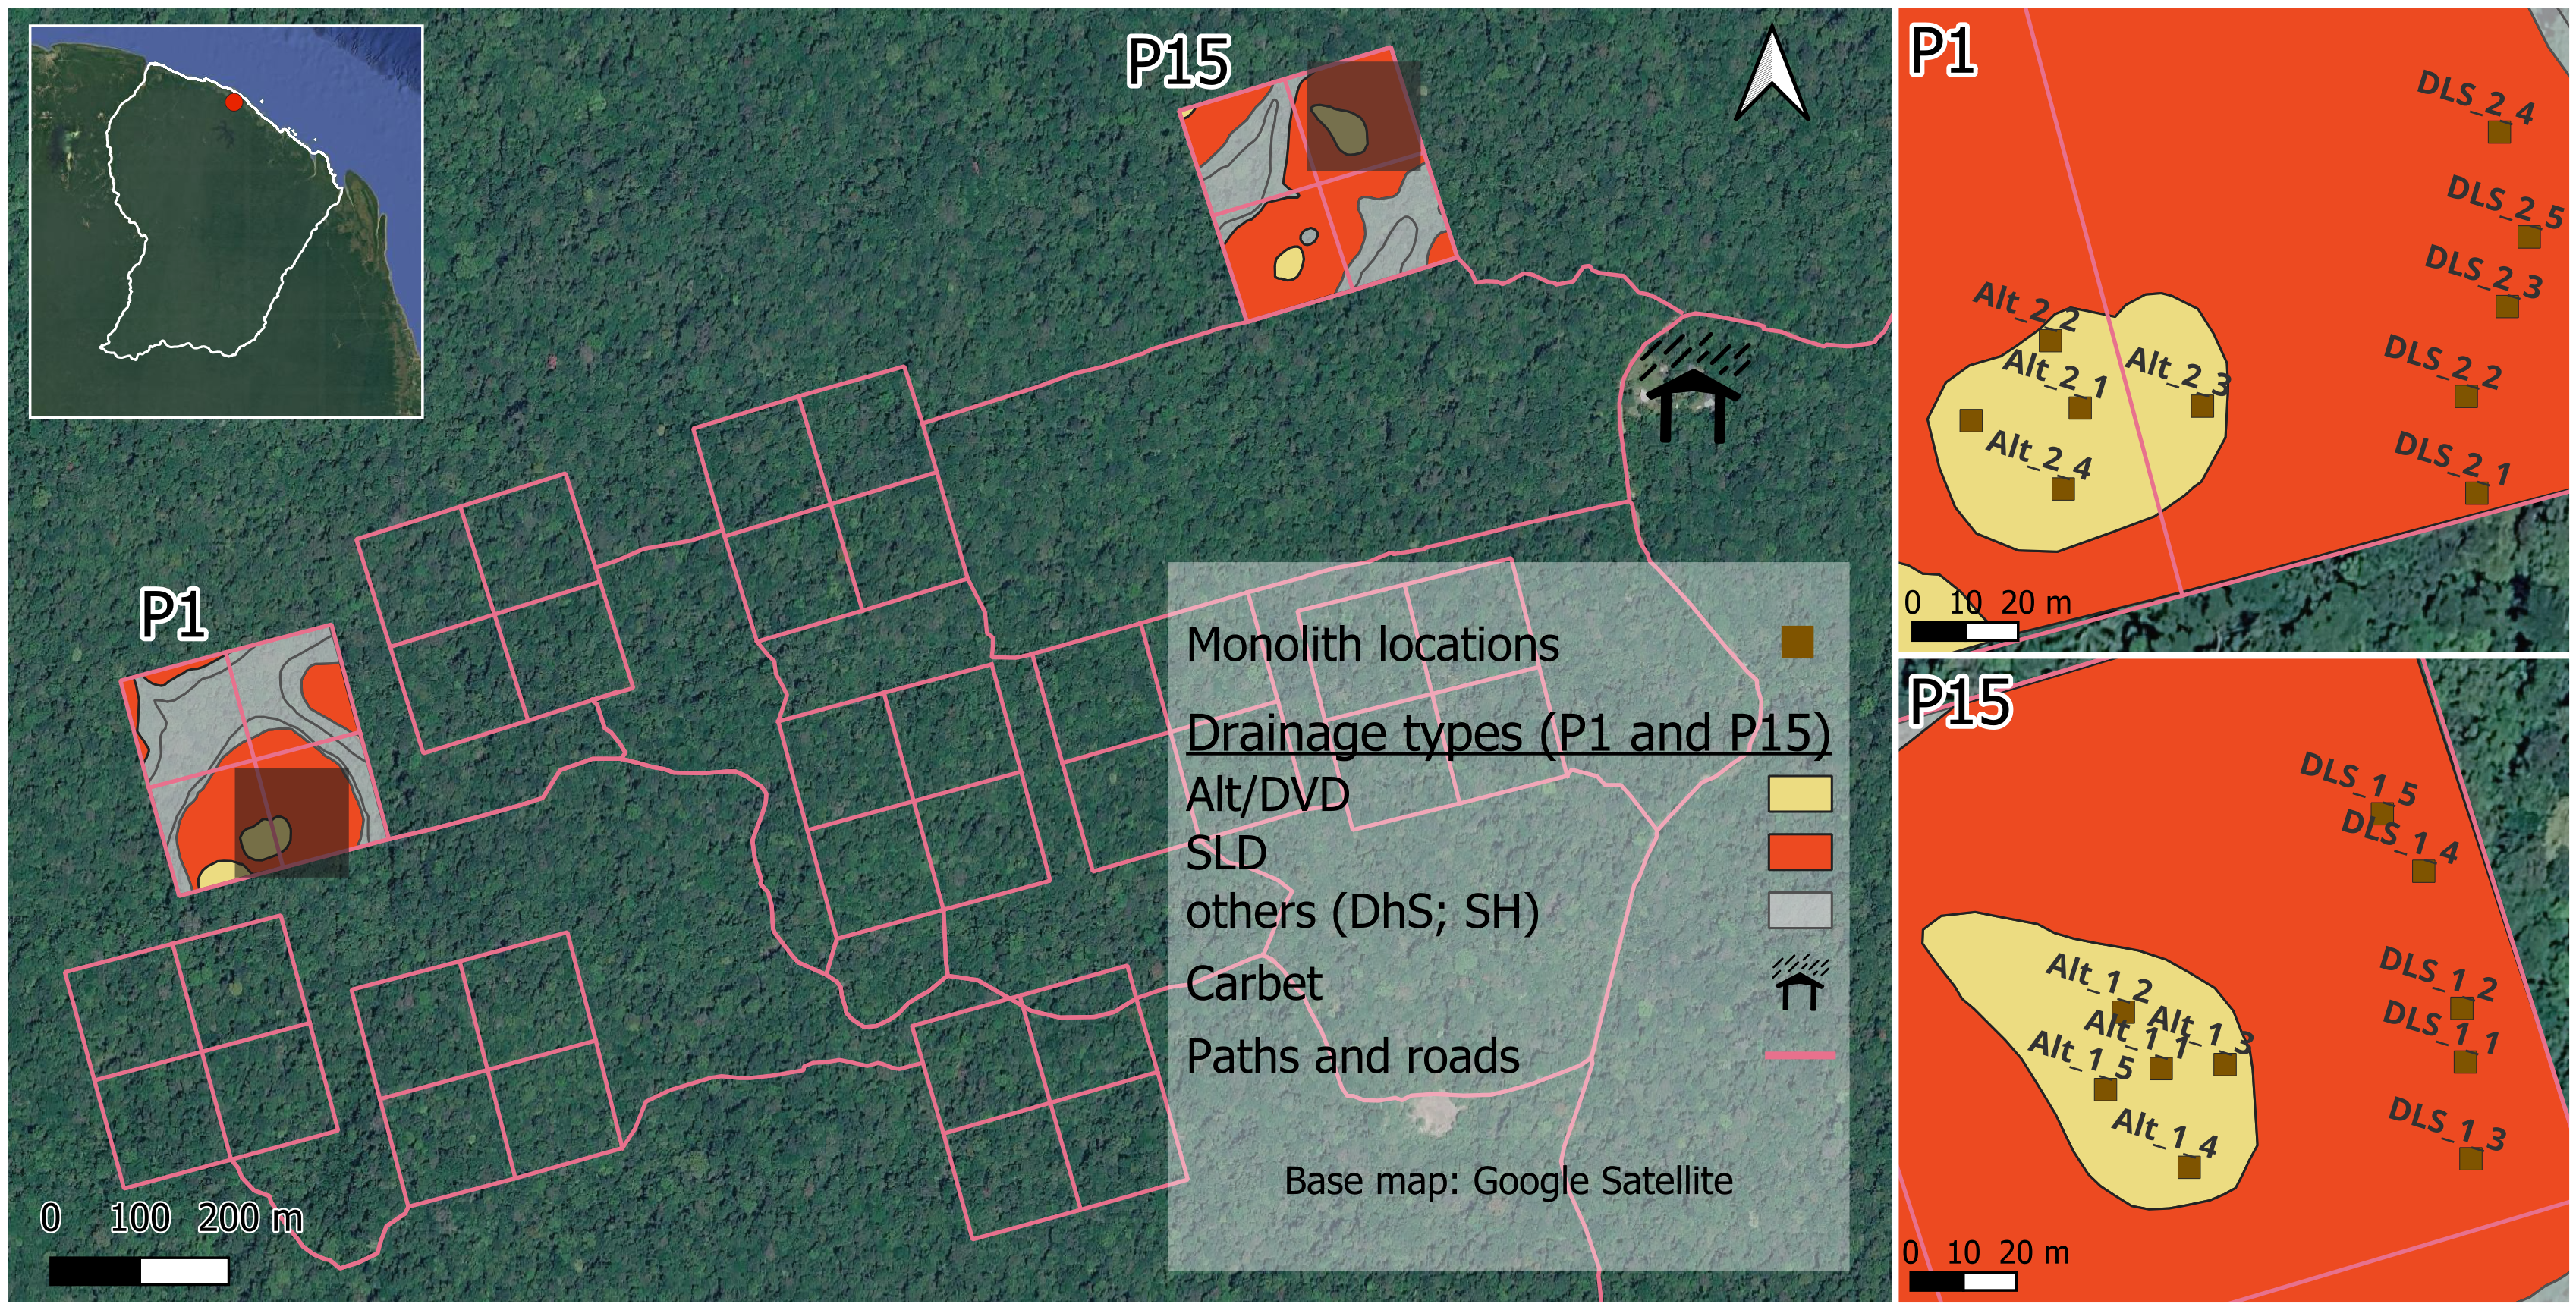
\includegraphics[width=1\linewidth,height=\textheight,keepaspectratio]{images/overview_paracou.png}

\normalsize

}

\caption{\label{fig-map}Overview map of Paracou with the sampling
locations. Location of right panels shown by grey squares. White lines
on the right panels represent altitude isolines.}

\end{figure*}%

PLACEHOLDER citation Ramos et al. (2025) or (Ramos et al., 2025), or
Freycon et al. (2003) or Pavlíček \& Csuzdi (2012)

\subsection{Sampling and
Identification}\label{sampling-and-identification}

text

\subsection{Statistical analysis}\label{statistical-analysis}

negative binomial (NB2) and Poisson tested

\subsubsection{Explorative Analysis}\label{explorative-analysis}

text

\subsubsection{Analysis of Abundances (Generalized Linear Mixed
Models)}\label{analysis-of-abundances-generalized-linear-mixed-models}

text

\subsubsection{Analysis of Community Composition
(PERMANOVA)}\label{analysis-of-community-composition-permanova}

text

\section{Results}\label{results}

\subsection{General}\label{general}

Densities by soil type and layer Figure~\ref{fig-density}

\begin{figure}

\centering{

\scriptsize

\pandocbounded{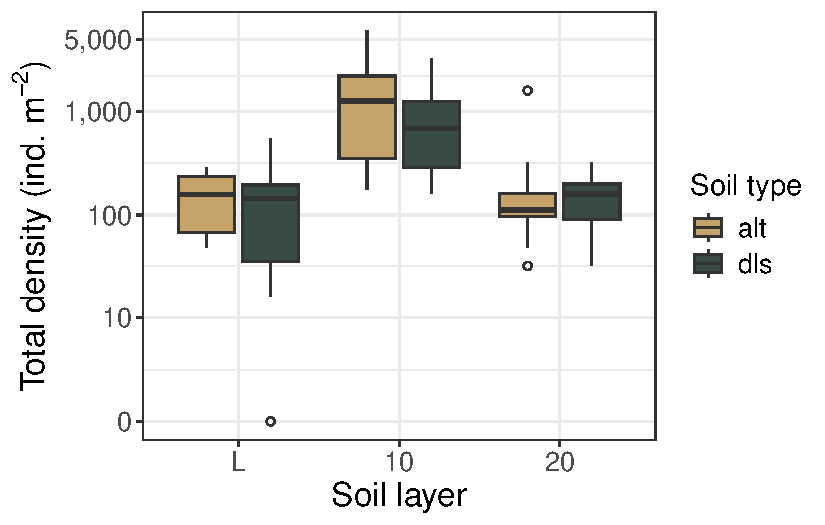
\includegraphics[keepaspectratio]{index_files/figure-pdf/Total macrofauna density boxplot FIGURE-1.pdf}}

\normalsize

}

\caption{\label{fig-density}Boxplot with total macrofauna densities by
soil type and layer. y-axis is logarithmic.}

\end{figure}%

Relative composition of community abundances Figure~\ref{fig-comp}

\begin{figure}

\centering{

\scriptsize

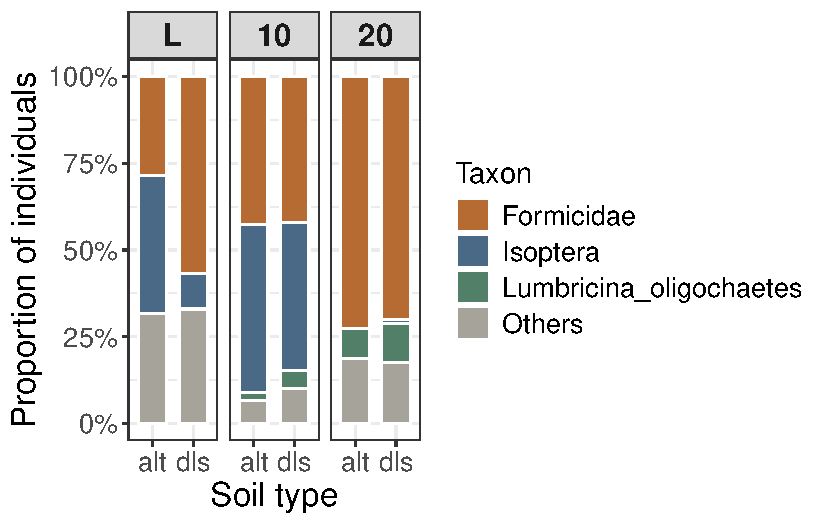
\includegraphics[width=1\linewidth,height=\textheight,keepaspectratio]{index_files/figure-pdf/Composition FIGURE-1.pdf}

\normalsize

}

\caption{\label{fig-comp}Relative composition of macrofaunal community
abundances by soil type and layer.}

\end{figure}%

Explorative ordination PCA Figure~\ref{fig-pca}

\begin{figure}

\centering{

\scriptsize

\pandocbounded{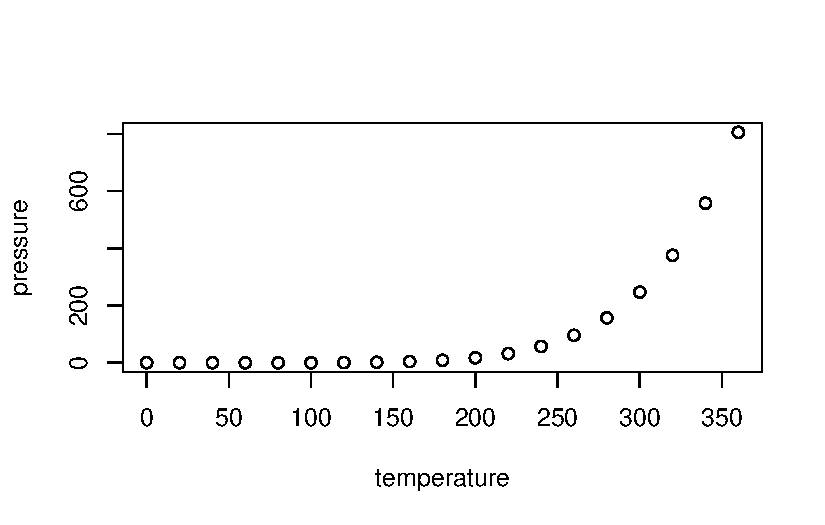
\includegraphics[keepaspectratio]{index_files/figure-pdf/PCA FIGURE-1.pdf}}

\normalsize

}

\caption{\label{fig-pca}PCA ordination based on Hellinger-transformed
community matrix. First two dimensions are presented. Only taxa with
cos² \textgreater{} 0.1 are presented.}

\end{figure}%

\subsection{GLMM}\label{glmm}

Effects of soil type and layer were tested on global, ant, termite and
earthworm abundances. All retained models described below are listed in
Table~\ref{tbl-models}.

\subsubsection{Global Abundance}\label{global-abundance}

Type II Wald chi-square tests revealed a highly significant effect of
soil layer on total soil macrofauna abundance (\(\chi^2\) = 106.85, df =
2, p \textless{} 0.001). The effect of soil type was not significant
(\(\chi^2\) = 0.52, df = 1, p = 0.469). Estimated random-effect variance
(monolith) was 0.437 (SD = 0.661), indicating variation in baseline
macrofauna abundance among monoliths.

Pairwise comparisons with Tukey adjustment (Table~\ref{tbl-pairwise})
showed that macrofauna abundance was significantly higher in layer 10
than in layers L (7.42 times) and 20 (6.18 times), while no significant
difference was found between layers L and 20 (p = 0.714).

\subsubsection{Formicidae}\label{formicidae}

Type II Wald chi-square tests revealed a highly significant effect of
soil layer on ant abundance (\(\chi^2\) = 28.00, df = 2, p \textless{}
0.001). The effect of soil type was not significant (\(\chi^2\) = 0.48,
df = 1, p = 0.486). The estimated random-effect variance for monolith
was 0.655 (SD = 0.810), indicating variation in baseline ant abundance
among monoliths. Quantile deviation was detected in the DHARMa residuals
for the presented model. Specifically, upper quantile deviated
significantly and thus relatively high-abundance observations may not be
adequately captured by the model. Since the diagnostics did not indicate
deviations regarding dispersion, zero-inflation, uniformity as well
outliers, and the model has the best AIC support, it was retained,
regardless.

Pairwise comparisons with Tukey adjustment (Table~\ref{tbl-pairwise})
showed that ant abundance was significantly higher in layer 10 than in
layer L (5.05 times) and layer 20 (3.27 times), while no significant
difference was found between layers L and 20 (p = 0.3995).

\subsubsection{Isoptera}\label{isoptera}

Type II Wald chi-square tests revealed a highly significant effect of
soil layer on termite abundance (\(\chi^2\) = 36.56, df = 2, p
\textless{} 0.001). The effect of soil type was not significant
(\(\chi^2\) = 0.89, df = 1, p = 0.347). The estimated random-effect
variance for monolith was effectively zero (\(8.22 \times 10^{-9}\); SD
= 0.00009), indicating virtually no remaining variation in baseline
termite abundance among monoliths after accounting for the fixed
effects.

Pairwise comparisons with Tukey adjustment (Table~\ref{tbl-pairwise})
showed that termite abundance was significantly higher in layer 10 than
in layer L (18.08 times) and layer 20 (745.48 times; estimated richness
for 20 nearing zero). Abundance was also significantly higher in layer L
than in layer 20 (41.23 times; all p \leq 0.0073).

\begin{table*}

\caption{\label{tbl-pairwise}Pairwise emmeans comparisons of abundance
by layer for total macrofauna, ants (Formicidae) and termites
(Isoptera).}

\centering{

\fontsize{8.0pt}{9.0pt}\selectfont
\begin{tabular*}{\linewidth}{@{\extracolsep{\fill}}ccccc}
\toprule
Taxon & Comparison & Abundance ratio & z-ratio & Adjusted p-value \\ 
\midrule\addlinespace[2.5pt]
Total macrofauna & L - 10 & 0.13 & -9.12 & \textless{}0.0001*** \\ 
Total macrofauna & L - 20 & 0.83 & -0.78 & 0.713689 \\ 
Total macrofauna & 10 - 20 & 6.18 & 8.34 & \textless{}0.0001*** \\ 
Ants (Formicidae) & L - 10 & 0.20 & -4.96 & \textless{}0.0001*** \\ 
Ants (Formicidae) & L - 20 & 0.65 & -1.29 & 0.399482 \\ 
Ants (Formicidae) & 10 - 20 & 3.27 & 3.84 & 0.000363*** \\ 
Termites (Isoptera) & L - 10 & 0.06 & -4.06 & 0.000145*** \\ 
Termites (Isoptera) & L - 20 & 41.23 & 3.01 & 0.007262** \\ 
Termites (Isoptera) & 10 - 20 & 745.48 & 5.42 & \textless{}0.0001*** \\ 
\bottomrule
\end{tabular*}
\begin{minipage}{\linewidth}
\vspace{.05em}
Abundance ratios are exponentiated log-scale contrasts. Significance levels: * p \textless{} 0.05; ** p \textless{} 0.01; *** p \textless{} 0.001. P-values adjusted using the Tukey method within each taxon.\\
\end{minipage}

}

\end{table*}%

\subsubsection{Lumbricina Oligochaetes}\label{lumbricina-oligochaetes}

Type II Wald chi-square tests indicated a significant effect of soil
layer on earthworm abundance (\(\chi^2\) = 12.69), df = 2, p = 0.0018),
whereas soil type had no significant effect (\(\chi^2\) = 0.35), df = 1,
p = 0.557). Pairwise comparisons showed significantly higher earthworm
abundance in layer 10 compared to layer 20 (2.31 times higher). No
significant differences were detected between layer L and the other
layers. However, no earthworms were recorded in layer L, resulting in
unstable model estimates and unbounded confidence intervals for this
layer. The Estimated random-effect variance for monoliths was 0.510 (SD
= 0.714)

\begin{table*}

\caption{\label{tbl-models}Summary of retained GLMMs for global
abundance, ants (Formicidae), termites (Isoptera) and earthworms
(Lumbricina oligochaetes). ADD MORE DESCRIPTION HERE}

\centering{

\fontsize{8.0pt}{9.0pt}\selectfont
\begin{tabular*}{\linewidth}{@{\extracolsep{\fill}}cccccc}
\toprule
Response & Distribution & Predictor & Chi-square & df & p-value \\ 
\midrule\addlinespace[2.5pt]
Total macrofauna & Negative binomial & soil\_type & 0.52 & 1 & 0.46933 \\ 
Total macrofauna & Negative binomial & layer & 106.85 & 2 & \textless{}0.0001*** \\ 
Ants & Negative binomial & soil\_type & 0.48 & 1 & 0.48633 \\ 
Ants & Negative binomial & layer & 28.00 & 2 & \textless{}0.0001*** \\ 
Termites & Negative binomial & soil\_type & 0.89 & 1 & 0.34664 \\ 
Termites & Negative binomial & layer & 36.56 & 2 & \textless{}0.0001*** \\ 
Earthworms & Poisson & soil\_type & 0.35 & 1 & 0.55692 \\ 
Earthworms & Poisson & layer & 12.69 & 2 & 0.00176** \\ 
\bottomrule
\end{tabular*}
\begin{minipage}{\linewidth}
\vspace{.05em}
Type II Wald chi-square tests. All models included soil type and soil layer as fixed effects and monolith ID as a random intercept. Significance levels: * p \textless{} 0.05; ** p \textless{} 0.01; *** p \textless{} 0.001\\
\end{minipage}

}

\end{table*}%

\subsection{PERMANOVA}\label{permanova}

PERMANOVA did not show a significant difference in macrofaunal community
composition between soil types (F = 1.68, R² = 0.085, p = 0.139). The
test for homogeneity of multivariate dispersion was also non-significant
(F = 0.11, p = 0.742), indicating no detectable difference in
within-group dispersion between soil types. Layers were aggregated per
monolith to account for spatial dependence.

PERMANOVA revealed a significant effect of soil layer on macrofauna
community composition (Bray--Curtis dissimilarity: F = 5.46, R² = 0.163,
p = 0.0001). Soil layer explained around 16.3\% of variation in the
community composition, indicating that macrofauna community composition
differed significantly among layers. Permutation was restricted within
monolith to account for spatial dependence of layers. Homogeneity of
multivariate dispersion was assessed using a permutation test based on
betadisper. No significant differences in dispersion were detected for
soil layers (F = 0.75, p = 0.321), suggesting that the PERMANOVA result
was not driven by differences in within-group dispersion.

Pairwise PERMANOVA suggests significant differences in macrofauna
community composition for all soil layers (Table~\ref{tbl-permanova}).
Significant differences were observed between L and 10 (F = 6.05, R² =
0.141, adjusted p = 0.0003), L and 20 (F = 4.55, R² = 0.110, adjusted p
= 0.0003), and 10 and 20 (F = 5.76, R² = 0.132, adjusted p = 0.0012),
using Bonferroni correction.

\begin{table}

\caption{\label{tbl-permanova}Pairwise PERMANOVA for community
composition comparisons between layers.}

\centering{

\fontsize{8.0pt}{9.0pt}\selectfont
\begin{tabular*}{\linewidth}{@{\extracolsep{\fill}}cccc}
\toprule
Comparison & F-statistic & R² & Adjusted p-value \\ 
\midrule\addlinespace[2.5pt]
L - 10 & 6.05 & 0.141 & 0.0003*** \\ 
L - 20 & 4.55 & 0.110 & 0.0003*** \\ 
10 - 20 & 5.76 & 0.132 & 0.0021** \\ 
\bottomrule
\end{tabular*}
\begin{minipage}{\linewidth}
\vspace{.05em}
Significance levels: * p \textless{} 0.05; ** p \textless{} 0.01; *** p \textless{} 0.001; p-values adjusted using Bonferroni method\\
\end{minipage}

}

\end{table}%

\begin{figure}

\centering{

\scriptsize

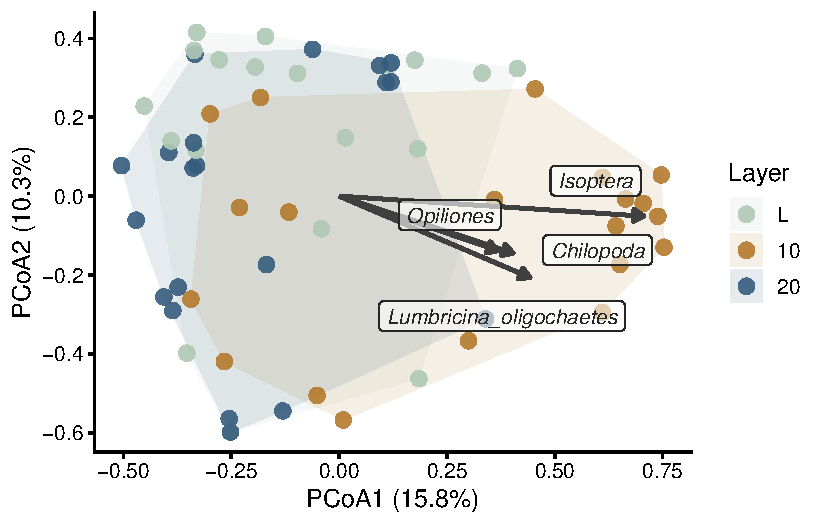
\includegraphics[width=1\linewidth,height=\textheight,keepaspectratio]{index_files/figure-pdf/PCoA FIGURE-1.pdf}

\normalsize

}

\caption{\label{fig-pcoa}Bray-Curtis PCoA for layers here}

\end{figure}%

\section{Discussion}\label{discussion}

text

\section{Conclusion}\label{conclusion}

text

\section*{References}\label{bibliography}
\addcontentsline{toc}{section}{References}

\protect\phantomsection\label{refs}
\begin{CSLReferences}{1}{0}
\bibitem[\citeproctext]{ref-Freycon2003}
Freycon, V., Sabatier, D., Paget, D., \& Ferry, B. (2003). Influence du
sol sur la végétation arborescente en forêt guyanaise : État des
connaissances. \emph{Revue Forestière Française}, 60--73.
\url{https://doi.org/10.4267/2042/5787}

\bibitem[\citeproctext]{ref-Pavlicek2012}
Pavlíček, T., \& Csuzdi, C. (2012). Earthworm fauna of {French Guiana}:
({Oligochaeta}). \emph{Zoology in the Middle East}, \emph{58}(sup4),
107--110. \url{https://doi.org/10.1080/09397140.2012.10648991}

\bibitem[\citeproctext]{ref-Ramos2025}
Ramos, A. P. D., Lima, S. S. D., Ferreira, C. D. S., Pinto, L. A. R. D.
S., Ferreira, R., Dias, A., Matos, P. S., \& Pereira, M. G. (2025).
Macrofauna and soil properties in agroforestry system and secondary
forest. \emph{Revista Brasileira de Ciência do Solo}, \emph{49},
e0240091. \url{https://doi.org/10.36783/18069657rbcs20240091}

\end{CSLReferences}




\end{document}
